\section{Introduction}

\begin{figure*}[t]
\centering
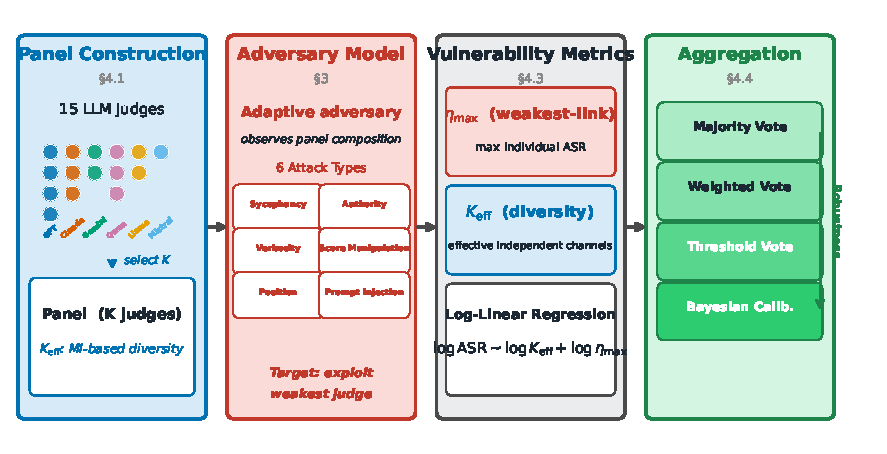
\includegraphics[width=\textwidth]{figures/fig_framework.pdf}
\caption{Predictor relevance patterns across panel sizes. \textbf{(a)}~In small panels ($K{=}3$), a single vulnerable judge (red) can flip the majority; individual weakness ($\eta_{\max}$) is the stronger predictor ($\hat{\beta}_{\mathrm{std}}{=}0.243$). \textbf{(b)}~As panel size increases, $\eta_{\max}$'s relevance decreases. \textbf{(c)}~At $K{\geq}5$, $K_{\mathrm{eff}}$'s pooled coefficient ($\hat{\beta}_{\mathrm{std}}{=}0.286$--$0.353$) remains positive while $\eta_{\max}$ CI crosses zero. Bottom bars show relative predictive weight.}
\label{fig:framework}
\end{figure*}

The widespread adoption of multi-judge panels for LLM evaluation rests on an untested assumption: that aggregating diverse judges provides robust defense against adversarial manipulation. After \citet{zheng2023judging} showed that individual LLM judges can rival human annotators, subsequent work exposed systematic vulnerabilities (position bias, verbosity preferences, and sycophancy) that compromise any single judge \citep{wang2023fair}, motivating majority-vote aggregation inspired by Byzantine fault tolerance (BFT) \citep{lamport1982byzantine,castro1999practical}. A recent systematization reports that 7-model committees reduce attack success rates (ASR) from 50--68\% to 10--19\% \citep{almasoud2026security}, reinforcing the belief that diversity is the key ingredient for secure evaluation.

This framing, however, conflates two distinct sources of robustness: the quality of individual judges and the independence among them. Evaluation adversaries manipulate inputs rather than controlling nodes, and shared pretraining corpora create correlated failures that violate the independence assumption underlying both classical fault tolerance and recent information-theoretic evaluation frameworks \citep{schneier2000secrets,kaneko2025bits,turkmen2026ensemble}. Within-family error correlations substantially exceed cross-family values \citep{kim2025correlated}, and panel accuracy saturates at moderate sizes \citep{yang2026diversity}, suggesting that simply scaling panel size yields diminishing returns. More critically, diversity and capability are structurally confounded: expanding family coverage inevitably introduces weaker judges, so the protective effect attributed to diversity may instead reflect a capability cost. No existing work examines how these two factors relate across panel sizes.

We address this gap by regressing panel vulnerability on two predictors (Figure~\ref{fig:framework}): weakest-link susceptibility ($\eta_{\max}$, the maximum individual attack success rate in a panel) and a pairwise-MI diversity index ($K_{\mathrm{eff}}$). Controlled experiments across 15 models (9 API, 6 local quantized), $K \in \{3,5,7\}$, six attack types, and two multiple-choice benchmarks (MMLU, ARC) reveal two consistent patterns.

First, $\eta_{\max}$ is significant at $K{=}3$ (meta-analytic pooled standardized coefficient $\hat{\beta}_{\mathrm{std}}{=}0.243$; \S\ref{sec:stat_framework}) but becomes non-significant at $K{\geq}5$ ($\hat{\beta}_{\mathrm{std}}$: $0.091$, $0.086$; confidence interval [CI] crosses zero). Second, $K_{\mathrm{eff}}$'s positive association with vulnerability persists across all panel sizes (pooled $\hat{\beta}_{\mathrm{std}}$: $0.286$--$0.353$, CI excluding zero), though the diversity--capability confound ($r{=}0.70$--$0.81$) precludes causal interpretation: in 69\% of conditions, the confound alone could account for the observed association. The pattern reverses for position bias, where diversity \emph{reduces} vulnerability, consistent with the Condorcet intuition for shared-bias attacks.

These findings yield three contributions:
\begin{enumerate}
\item \textbf{Diversity--vulnerability association under confound.} Diversity and vulnerability covary positively (pooled $\hat{\beta}_{\mathrm{std}}$: $0.286$--$0.353$, CI excludes zero), but both are confounded by capability ($r{=}0.70$--$0.81$); the association partially survives capability-matched subsampling (Pool~A, defined in \S\ref{sec:analysis}; $r{=}0.50$). Position bias is the exception ($\hat{\beta}_{\mathrm{std}} < 0$; \S\ref{sec:gam_taxonomy}).
\item \textbf{Weakest-link significance transition.} $\eta_{\max}$ is significant at $K{=}3$ (pooled $\hat{\beta}_{\mathrm{std}}{=}0.243$) but non-significant at $K{\geq}5$ ($0.091$, $0.086$; CI crosses zero). $K_{\mathrm{eff}}$'s pooled coefficient remains positive ($0.286$--$0.353$, CI excluding zero); significance trajectory is metric-dependent (\S\ref{sec:cross_k}).
\item \textbf{Aggregation as predictability control.} Aggregation rules modulate variance explained ($R^2$: threshold 0.75, Bayesian 0.14); Bayesian calibration attenuates $K_{\mathrm{eff}}$ but $\eta_{\max}$ persists (\S\ref{sec:aggregation}).
\end{enumerate}

All findings are associational; the diversity--capability confound (\S\ref{sec:analysis}) precludes causal claims.
